% The document class supplies options to control rendering of some standard
% features in the result.  The goal is for uniform style, so some attention 
% to detail is *vital* with all fields.  Each field (i.e., text inside the
% curly braces below, so the MEng text inside {MEng} for instance) should 
% take into account the following:
%
% - author name       should be formatted as "FirstName LastName"
%   (not "Initial LastName" for example),
% - supervisor name   should be formatted as "Title FirstName LastName"
%   (where Title is "Dr." or "Prof." for example),
% - degree programme  should be "BSc", "MEng", "MSci", "MSc" or "PhD",
% - dissertation title should be correctly capitalised (plus you can have
%   an optional sub-title if appropriate, or leave this field blank),
% - dissertation type should be formatted as one of the following:
%   * for the MEng degree programme either "enterprise" or "research" to
%     reflect the stream,
%   * for the MSc  degree programme "$X/Y/Z$" for a project deemed to be
%     X%, Y% and Z% of type I, II and III.
% - year              should be formatted as a 4-digit year of submission
%   (so 2014 rather than the accademic year, say 2013/14 say).

\documentclass[ % the name of the author
author={Dillon Keith Diep [INCOMPLETE DRAFT, NOT FOR SUBMISSION]},
% the name of the supervisor
supervisor={Dr. Carl Henrik Ek},
% the degree programme
degree={MEng},
% the dissertation    title (which cannot be blank)
title={ARt-CG:},
% the dissertation subtitle (which can    be blank)
subtitle={Assisted Real-time Content Generation of 3D Hair by Learning Manifolds},
% the dissertation     type
type={Research},
% the year of submission
year={2014} ]{dissertation}
\begin{document}
% =============================================================================

% This section simply introduces the structural guidelines.  It can clearly
% be deleted (or commented out) if you use the file as a template for your
% own dissertation: everything following it is in the correct order to use 
% as is.

% =============================================================================

% This macro creates the standard UoB title page by using information drawn
% from the document class (meaning it is vital you select the correct degree 
% title and so on).

\maketitle

% After the title page (which is a special case in that it is not numbered)
% comes the front matter or preliminaries; this macro signals the start of
% such content, meaning the pages are numbered with Roman numerals.

\frontmatter

% This macro creates the standard UoB declaration; on the printed hard-copy,
% this must be physically signed by the author in the space indicated.

\makedecl

% LaTeX automatically generates a table of contents, plus associated lists 
% of figures, tables and algorithms.  The former is a compulsory part of the
% dissertation, but if you do not require the latter they can be suppressed
% by simply commenting out the associated macro.

\tableofcontents
\listoffigures
\listoftables
\listofalgorithms
\lstlistoflistings

% The following sections are part of the front matter, but are not generated
% automatically by LaTeX; the use of \chapter* means they are not numbered.

% -----------------------------------------------------------------------------

\chapter*{Executive Summary}

{\bf A compulsory section, of at most $1$ page} 
\vspace{1cm} 

\noindent
The topic of this dissertation explores assisted content generation by training generative models using unsupervised machine learning for the production of 3D hair geometry. The research hypothesis of this study is that non-linear probabilistic principal component analysis with the Gaussian Process Latent Variable Model is applicable for improving the creative production workflow of complex 3D hair geometry for humanoids.

Production of 3D virtual worlds is a time-consuming and costly process that also demand expert knowledge. 3D assets encompass a vast range of applications, ranging from simulations and research, to contributing towards the functioning of many businesses. The production of 3D assets impacts many industries including engineering, medicine, and the provisioning of entertainment. One particular task is the creation of 3D hair geometry for humanoid characters. Creating 3D hair is arduous as hair structure is a complex system containing much interdependence between components.

Machine learning applications typically use large data sets for training on problems that often have a concise answer for a given prediction. The application of machine learning to enhance production for creative work is an exciting field that tackles novel challenges: artistic products tend to have small sets of data available and evaluation of quality is subjective. Given the same input, acceptable solutions can vary significantly. The outlined peculiarities of applying machine learning for 3D mesh data establish a unique field of problems to investigate.

Existing tools for 3D modelling have remained mostly static in the paradigm of approach over the past several decades. Automation through methods such as procedural generation can produce output much faster, but the lack of control over the final result makes it less desirable than traditional methods of 3D modelling. The focus of this project is to formulate a revolutionary approach that offers an alternative work-flow which could potentially improve the efficacy of producing 3D hair geometry through unsupervised training of generative models.

Deliverables:
\begin{quote}
	\noindent
	\begin{itemize}
		\item Formulation of a generative model for 3D humanoid hair structure.
		\item Resolving the alignment problem by approximating raw input data using a generative model.
		\item Learning a low dimension latent-space of high dimensional hair structure data.
		\item Investigated the performance of various kernels for high dimensional training data.
		\item Implemented an add-on package for a 3D production program, Blender.
		\begin{itemize}
			\item The implementation creates guiding splines that are useful for generating hair geometry.
			\item Appropriate for small training set that is practical for content creators.
			\item Real-time performance that matches state of the art non-learning tools.
			\item Functionality to records user activity for analysis.
		\end{itemize}
		\item Acquired data for evaluation of the research hypothesis.
	\end{itemize}
\end{quote}

% -----------------------------------------------------------------------------

\chapter*{Supporting Technologies}

{\bf A compulsory section, of at most $1$ page}
\vspace{1cm} 

\noindent
This section should present a detailed summary, in bullet point form, 
of any third-party resources (e.g., hardware and software components) 
used during the project.  Use of such resources is always perfectly 
acceptable: the goal of this section is simply to be clear about how
and where they are used, so that a clear assessment of your work can
result.  The content can focus on the project topic itself (rather,
for example, than including ``I used \mbox{\LaTeX} to prepare my 
dissertation''); an example is as follows:

\begin{quote}
	\noindent
	\begin{itemize}
		\item I used the Java {\tt BigInteger} class to support my implementation 
		of RSA.
		\item I used a parts of the OpenCV computer vision library to capture 
		images from a camera, and for various standard operations (e.g., 
		threshold, edge detection).
		\item I used an FPGA device supplied by the Department, and altered it 
		to support an open-source UART core obtained from 
		\url{http://opencores.org/}.
		\item The web-interface component of my system was implemented by 
		extending the open-source WordPress software available from
		\url{http://wordpress.org/}.
	\end{itemize}
\end{quote}

% -----------------------------------------------------------------------------

\chapter*{Notation and Acronyms}

{\bf An optional section, of roughly $1$ or $2$ pages}
\vspace{1cm} 

\noindent
Any well written document will introduce notation and acronyms before
their use, {\em even if} they are standard in some way: this ensures 
any reader can understand the resulting self-contained content.  

Said introduction can exist within the dissertation itself, wherever 
that is appropriate.  For an acronym, this is typically achieved at 
the first point of use via ``Advanced Encryption Standard (AES)'' or 
similar, noting the capitalisation of relevant letters.  However, it 
can be useful to include an additional, dedicated list at the start 
of the dissertation; the advantage of doing so is that you cannot 
mistakenly use an acronym before defining it.  A limited example is 
as follows:

\begin{quote}
	\noindent
	\begin{tabular}{lcl}
		AES                 &:     & Advanced Encryption Standard                                         \\
		DES                 &:     & Data Encryption Standard                                             \\
		&\vdots&                                                                      \\
		${\mathcal H}( x )$ &:     & the Hamming weight of $x$                                            \\
		${\mathbb  F}_q$    &:     & a finite field with $q$ elements                                     \\
		$x_i$               &:     & the $i$-th bit of some binary sequence $x$, st. $x_i \in \{ 0, 1 \}$ \\
	\end{tabular}
\end{quote}

{ \color{red}
$x$ scalar

$\bm{x}$ column vector

$\bm{x}^T$ row vector, superscript T denotes transpose

$\bm{X}$ matrix

$\bm{I}$ identity matrix
}

% -----------------------------------------------------------------------------

\chapter*{Acknowledgements}

{\bf An optional section, of at most $1$ page}
\vspace{1cm} 

\noindent
It is common practice (although totally optional) to acknowledge any
third-party advice, contribution or influence you have found useful
during your work.  Examples include support from friends or family, 
the input of your Supervisor and/or Advisor, external organisations 
or persons who  have supplied resources of some kind (e.g., funding, 
advice or time), and so on.

% =============================================================================

% After the front matter comes a number of chapters; under each chapter,
% sections, subsections and even subsubsections are permissible.  The
% pages in this part are numbered with Arabic numerals.  Note that:
%
% - A reference point can be marked using \label{XXX}, and then later
%   referred to via \ref{XXX}; for example Chapter\ref{chap:context}.
% - The chapters are presented here in one file; this can become hard
%   to manage.  An alternative is to save the content in seprate files
%   the use \input{XXX} to import it, which acts like the #include
%   directive in C.

\mainmatter

% -----------------------------------------------------------------------------

\chapter{Contextual Background}
\label{chap:context}

\section{Production of 3D Content}
There are many representations of 3D objects in computer graphics. A point cloud representation is a collection of points (vertices) that describe surface geometry. Range images map pixels of a depth image to a set of points in the scene. Voxels are unit cubes, corresponding to the concept of pixels, a collection of voxels describe an object volumetrically. These representations are common when sampling raw geometric data using 3D scanning devices. Each  representation have advantages and disadvantages depending on the use case. It is possible to convert between representations, however, data loss may be incurred. The most precise representations are generally mathematical models such as NURBS (Non-uniform rational basis spline) - often applied in the CAD (Computer-Aided Design) industry. The most widely applied representation used for CGI (computer-generated imagery) are polygonal meshes.

In a production environment, it is straightforward to define geometry precisely to specified requirements as opposed to capturing examples. A polygon mesh is constructed of vertices, edges, and faces. The topology of a mesh concerns with the arrangement of its components, well-organised topology is required to maintain geometric qualities when processing the mesh with algorithmic operations. Polygon meshes are simple to define, yet combined with established techniques such as UV texture and normal mapping, are sufficiently expressive for visual purposes. Significant study has been conducted on the field of polygon meshes improve its versatility. In practice, polygon meshes are organised with quad-face topology (faces formed from four edges) during production. Quads conform better with editing tools and algorithms. The rendering pipeline often automatically converts polygon meshes to tri-faces (faces formed from three edges) as an optimisation process.

\subsection{3D Hair Geometry}
On average, a human is born with between 90,000 to 150,000 scalp hair follicles. \cite{hairfollicles} It is computationally very expensive to render and animate physically correct hair, but creative liberties have been taken to approximate, or stylise 3D hair such that it is both acceptable aesthetically and feasible in terms of performance. This study considers modelling of hair geometry, the motion of hair is assumed to be its default resting pose.

In recent years, impressive 3D hair solutions for real-time simulation of realistic hair and fur, such as \textit{NVIDIA HairWorks} and \textit{AMD TressFX} has emerged. These solutions, however, have limited application in comparison to their traditional counterpart of polygonal hair. It is often the case that texture-mapped polygonal hair is used as a fallback when advanced simulation fails. Realism is not necessarily always desirable, polygon hair can flexibly represent different art styles. In some cases, a blend of multiple representations are used to balance between cost and quality. 3D hair in cinematography with large budget can afford to render hair with much higher fidelity for important characters, but would still consider use efficient variants for scenarios such as crowd simulation. Ultimately, it can be observed that the representation of virtual hair generally follows a structure of splines with control points that define the overall organisation of strands or segments.

\begin{figure}[!h]
	\centering
	To add %*
	\caption{Image of hair geometry.}
	\label{fig}
\end{figure}

\section{Curse of Dimensionality}
The curse of dimensionality is a term coined by Bellman, \cite{curseofdyn} which refers to the phenomena where exhibited complexity of high-dimensional spaces grows exponentially greater than those of low-dimensionality. From the perspective of a 3D content creator, manipulating high-dimensional data such as hair geometry is a daunting task that becomes increasingly difficult as more detail is added. Computationally, algorithms scale far better with low-dimensional data, causing complex geometry such as hair to be challenging for machine learning methods.

\subsection{Procedural Generation and Automated Production}
Procedural generation techniques produce output that adhere to rules established by the generative model defined. Such techniques have been successfully applied for generation of terrains and city modelling. \cite{procedural1} Fractals and methods such as the Lindenmayer system has been used to produce patterns that resemble those observed in nature. \cite{lsystem} Automated techniques such as the ones discussed, however, are seldom used for modelling important objects with specific design. It is difficult to control the output of procedurally generated content without heavily restricting its capabilities. Automated methods that do not learn is cannot adapt to changing demands without reimplementation.


\section{Related Research of Machine Learning in Creative Fields}
The task of machine learning can be divided into three major paradigms: 
\begin{itemize}
	\item \textit{Supervised learning} is provided input training examples with desired outputs to learn the mapping of inputs to output.
	\item \textit{Unsupervised learning} is given only input data, the procedure learns structure of and relation between data.
	\item \textit{Reinforcement learning} seeks to iteratively improve a pool of solutions by simulating an environment that apply concepts inspired by the theory of evolution.
\end{itemize}
The role that learning methods play in both manufacturing and consumer application continue to grow, however, adoption has been slow for creative fields.  Generally, robust models improve in performance as more reliable data is obtained. Creative production values uniqueness and versatility, properties that cause difficulty in machine learning methods. Varying artistic styles in design complicate feature analysis and ambiguity of correctness is problematic when predicting an output.

To overcome the challenges of the scenario introduced above, dimensionality reduction through unsupervised learning with probabilistic latent variable models such as the Gaussian Process Latent Variable Model (GP-LVM) \cite{gplvm} present an opportunity to learn stylistic properties of design and predict multiple acceptable outputs by analysing the likelihood.
The following section will discuss related research conducted that also explores the idea of applying machine learning in creative fields.

\subsection{Style-Based Inverse Kinematics}
Style-based inverse kinematics introduced the Scaled Gaussian Process Latent Variable Model, based on GPLVM, to learn the probabilistic distribution of a 3D human posture model. \cite{styleik} Character posing from motion data is represented as a 42-dimensional feature vector that encapsulated joint information of a humanoid body. Learning a model of poses established the relation between joints and identified constraints exhibited in the training data - where unusual postures are given a lower likelihood rating.

\subsection{Latent Doodle Space}
A latent doodle space is the use of a low-dimension latent space that has been applied on simple line drawings. \cite{latentdoodle} The motivation of a latent doodle space is to generating new drawings that are inspired by the input data. There are two key phases to derive a latent doodle space: the first challenge is to identify line strokes within drawings, a latent variable method is then used to learn a latent space.

\subsection{Learning a Manifold of Fonts}
A study by Campbell \& Kautz presented a framework that learns the latent manifold of existing font styles. \cite{fontmanifold} The process involved universal parametrization of fonts to a polyline representation so that a distance measure is applicable and the generative model can interpolate between styles. Unsupervised learning with the GP-LVM model enabled rapid prototyping and non-experts could create font styles without experience on type design.

\subsection{Real-time Drawing Assistance through Crowd-sourcing}
Drawing assistance powered by large-scale crowd-sourcing explored the potential of data driven drawing to prompt for correction by achieving an artistic consensus. \cite{drawingassistance} A consensus is found by learning a correction vector field from training drawings. Stroke-correction is applied using the correction vector field to adjust user input dynamically.

\subsection{AutoHair}
Chai, et al introduced AutoHair, a method for automatic modelling of 3D hair from a portrait image. \cite{autohair} The approach extracts information from images and uses a database of hair meshes to construct a 3D representation of the information conveyed. A hierarchical deep neural network trained on annotated hair images learn to segment hair and estimate growth direction within portraits. Data-driven hair matching and modelling algorithm fit meshes from the database to parameters output by the neural net model to automatically produce 3D hair. The experiment developed a traversable hairstyle space of 50,000 hair models, using training images and 3D exemplars obtained from the internet.

\section{Motivation and Significance}
State of the art 3D production software such as AutoDesk Maya, 3DS Max, and Blender are advanced programs with sophisticated list of features. That said, such programs have extremely convoluted user interfaces, even the most experienced professionals do not recognise each and every tool available. The most versatile tools are generally the most basic that perform atomic changes as they are applicable in every scenario. Examples include selection of primitives such as vertices, edges, or faces and performing translation, rotation, and scaling. Sculpting tools move many data points simultaneously, they are often used for defining organic surfaces now that modern machines are sufficiently powerful. Experienced artists might search for an existing base mesh that is similar to start on, but it is not always the case that such a base mesh exists - there are also concerns for quality, such as poor topology. As the geometry becomes more detailed and well-defined, each alteration makes less impact and the space of sensible changes becomes smaller. The design and production of 3D geometry remains a slow and delicate process.

Virtual hair creation is a necessity for characters of CG movies and video games that are embedded within culture both economically and as entertainment. Specialised artists learn to be proficient with the design of hair, variety of styles, and techniques for creating them. Hair geometry is much more concentrated than other types, containing many data points that is exhausting to edit. Soft selection and sculpting tools are good enough for defining the structure but maintaining topology and issues such as overlapping surfaces are still problematic. Learning the relation of hair structure allows the potential of discovering new hairstyles.  It can also be used as a mean of rapidly generating initial base geometry that fits the target output better than existing geometry available. Generative methods could ensure a level of quality, clean topology that fits established specifications. Assisted content generation using machine learning provides a convenient, non-intrusive and intuitive method for rapidly generating new hair geometry from existing data.

%**Move to evaluation
The application of machine-learning based tools could enhance the workflow of professional users and improve the experience for non-expert consumers. Such tools integrate into the production environment to improve the efficiency of acquiring initial base geometry and visually compare designs during pre-production. Non-expert users receive the ability to produce 3D geometry without requiring to learn the intrinsics of traditional 3D modelling software. The rise of augmented reality and 3D printing inspires the development of generative tools that are intuitive and simplistic to use. Applications that allow users to create personal content could also integrate machine-learning based tools to prevent inappropriate or undesirable creation from being produced while providing options that surpass existing alternatives. An example would be avatar creation for many applications and video games. A space of reasonable options generated from predefined outputs by the developers will allow users to interpolate between sensible configurations, providing an excellent level of customisation while adhering to defined constraints.

\section{Challenges}
This study faces a number of challenges. Firstly, 3D meshes are difficult to compare. The training data in its raw form will have varying dimensions. Meshes can be viewed as samples of the true geometry, thus meshes that represent the same object could differ drastically in number of data points depending on its level of detail. Typical feature extraction methods do not work well on meshes as artistic products are sensitive to data loss - any change could affect the perception of final result drastically.

Another problem encountered is the lack of training data. Typical machine learning solutions use huge data sets in the order of hundreds of thousands for training, but for 3D meshes the expected size of readily available training data is much smaller. Public repositories of 3D polygonal hair are generally around a few thousand in size. \cite{tsr} Studios that store and organise past production could likely match the size of public repositories, depending on the size of the company. Private repositories of independent artists will rarely exceed the order of hundreds.

The application of machine learning methods must also account for subjectivity of evaluating artistic assets. The range of acceptable solutions is ambiguous, likened to how hair styles of characters can change drastically during the design phase, determining the threshold of acceptable solutions will be in itself a challenge to resolve.

As mentioned previously, 3D meshes are delicate and can easily be invalidated from small changes. Thus, reparations to ensure that the output of trained models are acceptable is a topic to explore.

In a production environment, the time required for a technique to return observable result directly affects throughput. For practical efficacy of assisted content generation, the technique should be reasonably fast in presenting observable output.

\section{Central Objectives}
%The aim of this study is ...
\begin{itemize}
	\item Resolving the alignment problem of 3D data through a representative generative model.
	\item Explore the application of GP-LVM for 3D hair geometry in a production pipeline.
	\item Investigate the use of latent variables for identifying stylistic properties of 3D hair geometry.
	\item Demonstrate the use of non-linear manifold to generate new hairstyles from training data.
	\item Enable an intuitive method for non-experts to create 3D hair geometry.
	\item Observable output demand performance close to real-time for practical use.
\end{itemize}

% -----------------------------------------------------------------------------

\chapter{Technical Background}
\label{chap:technical}

\section{Principal Component Analysis}
In multivariate analysis, principal component analysis (PCA) is a statistical technique used to perform linear dimensionality reduction. It was originally introduced by Pearson \cite{pca1901}, and independently developed by Hotelling \cite{pca1933}, where the standard algebraic derivation of PCA was presented in terms of a standardized linear projection.

Consider the properties that describe hair structure. Observable variables that can be measured include location, orientation, length, and colour. The data collected may indicate that some variables change together, this relation is measured as the covariance. The PCA technique searches for an ordered set of principal components that retain maximal variance. A principal component can be viewed as a combination of the observed variables. Should two observed variables strongly covary linearly, then it is plausible to describe the data with a single variable instead. The more linearly observed variables covary, the less information is lost from choosing a smaller set of principal components, thus effectively reducing dimensionality.

Given a set of $n$ observed $d$-dimensional data represented as a design matrix, $\bm{X=[x_1,...,x_n]}^T$, the $q$ principal components $\bm{w_j}$, $j \in {1,...,q}$, are the orthonormal axes with maximal variance retained. The first principal component is a linear function $\bm{\alpha}^T_1\bm{X}$ that retains most variance of $\bm{X}$, where $\bm{\alpha} = [\alpha_{11}, \alpha_{12}, ..., \alpha_{1n}]$ is a vector of $n$ constants such that:
$$\bm{\alpha}^T_1\bm{X}=\alpha_{11}\bm{x_1}+\alpha_{12}\bm{x_2}+...+\alpha_{1n}\bm{x_n} = \sum^n_{i=1}a_{1i}\bm{x_i}$$
The following principal components are found by looking for a linear function that is orthogonal to the selected principal components and retain maximum variance.

PCA can be performed by singular value decomposition (SVD) of $\bm{X}$ in matrix form, \cite{pca2002}
$$\bm{X=ULV}^T,$$
where given $r = r(\bm{X})$ denotes the rank of $\bm{X}$, then
$\bm{U} \in \Re^{n \times r}$ is a matrix of orthonormal columns that are the left singular vectors,
$\bm{L} \in \Re^{r \times r}$ is a diagonal matrix of the singular values of $\bm{X}$, and
$\bm{V} \in \Re^{d \times r}$ is a matrix of orthonormal columns that are the right singular vectors.

\section{Probabilistic Principal Component Analysis}
A limitation of standard PCA is the lack of a probabilistic solution. Tipping and Bishop introduced a probabilistic principal component analysis by constraining the noise distribution of a latent variable model to be Gaussian such that it is effectively equivalent when its marginal likelihood is maximised. \cite{ppca}

Suppose that the PCA is applied to a set of data that represents hair structure. Standard PCA searches for the orthonormal axes that retain maximal variance. Extrapolating values using the principal axes can infer new hairstyles, but only within a fixed style described by the principal axes. In the case of 3D content production, it is much more useful to have a selection of plausible designs to choose from. A probabilistic model of PCA will enable exploration of other potential linear embeddings of hair structure.


\subsection{The Gaussian Distribution}
The Gaussian (normal) distribution is a reasonable prior assumption for data that is subject to the central limit theorem, which states that as the sample size of a population tends to infinity, the distribution becomes increasingly Gaussian. \cite[p.78]{bishop}
A random variable $X$ that is normally distributed with mean $\mu$ and variance $\sigma^2$ is denoted as
$$X\sim\mathcal{N}(\mu, \sigma^2).$$
The Gaussian density for a single variable $y$ is expressed as \cite[p.78]{bishop}:
$$\mathcal{N}(y|\mu, \sigma^2)=\frac{1}{\sqrt{2\pi\sigma^2}}\exp\left(-\frac{(y-\mu)^2}{2\sigma^2}\right),$$
$$\mathcal{N}(y|\mu,\sigma^2) \equiv p(y|\mu,\sigma^2).$$

\subsubsection{Properties of Gaussian Distribution}
Notable properties of the Gaussian distribution that are useful include the summation (\ref{gd:sum}), scaling (\ref{gd:scale}), and product (\ref{gd:prod}) operation - all of which yields a result that is also a Gaussian distribution. \cite[p.200]{gp}
\begin{equation} \label{gd:sum}
\sum^n_{i=1}y_i\sim\mathcal{N}(\sum^n_{i=1}\mu_i,\sum^n_{i=1}\sigma^2_i)
\end{equation}

\begin{equation} \label{gd:scale}
wy\sim\mathcal{N}(w\mu,w^2\sigma^2)
\end{equation}

\begin{equation} \label{gd:prod}
\mathcal{N}(\bm{x|a},A)\mathcal{N}(\bm{x|b},B) = \mathcal{N}(\bm{a|b},A+B)\mathcal{N}(\bm{x}|\bm{c}, C),
\end{equation}
$$\bm{c}=C(A^{-1}\bm{a}+B^{-1}\bm{b}),$$
$$C = (A^{-1}+B^{-1})^{-1}).$$


\subsubsection{Multivariate Gaussian Distribution}
\noindent
Let $w$ and $h$ be jointly Gaussian distributed variables, if the variables are independent, then $p(w,h)=p(w)p(h)$.
The joint probability density is thus,
$$p(w,h)=\frac{1}{\sqrt{2\pi\sigma^2_1}\sqrt{2\pi\sigma^2_2}}\exp\left(-\frac{1}{2}\left(\frac{w-\mu_1)^2}{\sigma^2_1}+\frac{h-\mu_2)^2}{\sigma^2_2}\right)\right).$$
In matrix form, the joint probability is
$$p(w,h)=\frac{1}{2\pi\sqrt{\sigma^2_1\sigma^2_2}}\exp
\left(
-\frac{1}{2}
\left(
\left[
\begin{matrix}
w \\
h
\end{matrix}
\right]
-
\left[
\begin{matrix}
\mu_1 \\
\mu_2
\end{matrix}
\right]
\right)^T
\left[
\begin{matrix}
\sigma^2_1  &   0\\
0           &   \sigma^2_2
\end{matrix}
\right]
\left(
\left[
\begin{matrix}
w \\
h
\end{matrix}
\right]
-
\left[
\begin{matrix}
\mu_1 \\
\mu_2
\end{matrix}
\right]
\right)
\right).$$
For a $n$-dimensional vector $\bm{y}$, the joint probability density is expressed as
\begin{equation} \label{jointpd}
p(\bm{y})=\frac{1}{2\pi|\bm{D}|^{1/2}}\exp\left(-\frac{1}{2}(\bm{y}-\bm{\mu})^T\bm{D}^{-1}(\bm{y}-\bm{\mu})\right),
\end{equation}
where $\bm{D}\in\Re^{n \times 1}$ is the diagonal matrix of the variances $\Sigma$. \cite[p.78]{bishop}

\subsection{Latent Variable Models and Factor Analysis}
A latent variable model transforms a set of $n$ $d$-dimensional observed variables encoded as a design matrix, $\bm{Y}\in\Re^{n \times d}$, to a set of $n$ $q$-dimensional latent (unobserved) variables, $\bm{X}\in\Re^{n \times q}$. Latent variables are parsimonious, it is generally the case that $q \ll d$, explaining the original data with fewer variables. A notable latent variable model is that of factor analysis, one that assumes linearity in relation of the observed data set,
\begin{equation} \label{ppca:fa}
\bm{Y=WX+\mu+\epsilon}.
\end{equation}
$\bm{W}$ represents a matrix that specifies the linear relation between the observed data-space with the latent-space.
The parameter $\mu$ allows for non-zero mean, and the $\epsilon$ parameter represents noise within the model. Standard PCA can be viewed as a variant of factor analysis where the noise parameter is not accounted for. The maximum-likelihood estimates of $\bm{W}$ will thus generally not correspond to the principal subspace. 

\subsection{A Probabilistic Model for PCA}
Tipping and Bishop develop a latent variable model that performs principal component analysis by modelling the parameter $\epsilon$ of equation \ref{ppca:fa} as an isotropic, spherical Gaussian distribution $\mathcal{N}(\bm{0},\beta^{-1}\bm{I})$. Consider a design matrix of $n$ centred $d$-dimensional vectors $\bm{Y=[y_1,...,y_n]}^T$.
For each observed data point, $1 \leq i \leq n $, there is an associated $q$-dimensional latent variable $\bm{x_i}$.
The original data can be represented in terms of the latent variable with noise value,
$$\bm{y}_i=\bm{Wx}_i+\bm{\epsilon}_i.$$
A general representation for data with non-zero mean includes the mean parameter, $\bm{\mu}_i$,
$$\bm{y}_i=\bm{Wx}_i+\bm{\mu}_i+\bm{\epsilon}_i.$$
The matrix $\bm{W \in \Re^{d \times q}}$ represents the linear relationship between the latent-space with the  data-space. The noise values, $\epsilon_i \in \Re^{d \times 1}$, are sampled from a independent spherical Gaussian distribution, $\epsilon_i\sim\mathcal{N}(\bm{0, \beta^{-1}I})$.
The conditional probability distribution of a observed variables $\bm{y}_i$ given input variables $\bm{x}_i$ is thus Gaussian distributed as
\begin{equation} \label{ppca:conditional}
p(\bm{y}_i|\bm{x}_i)=\mathcal{N}(\bm{W\bm{x}_i+\bm{\mu}_i},\bm{\beta}^{-1}\bm{I}). 
\end{equation}
The marginal distribution over the latent variables are standard Gaussian, defined as $\bm{x}_i\sim\mathcal{N}(\bm{0},\bm{I})$. The marginal distribution for the observed data $\bm{y}_i$ is obtained by integrating out the latent variables.
From equation \ref{jointpd}, an arbitrary rotation matrix $\bm{R}^T\in\Re^{n \times n}$ can be applied to the basis, forming the correlated Gaussian,
$$p(\bm{y}_i)=\frac{1}{2\pi|\bm{D}|^{1/2}}\exp\left(-\frac{1}{2}(\bm{R}^T\bm{y}_i-\bm{R}^T\bm{\mu}_i)^T\bm{D}^{-1}(\bm{R}^T\bm{y}_i-\bm{R}^T\bm{\mu}_i)\right).$$
This gives an eigenvalue decomposition of the inverse covariance matrix, and thus the covariance matrix,
$$\bm{C}^{-1}=\bm{RD}^{-1}\bm{R}^T,$$
$$\bm{C}=\bm{RDR}^T.$$
As a consequence, we can derive that given $\bm{x}_i\sim\mathcal{N}(\bm{\mu}_i,\bm{\beta}^{-1})$ and $\bm{y}_i=\bm{Wx}_i$, then the distribution of the observed variables can be denoted as $\bm{y}_i\sim\mathcal{N}(\bm{W\mu}_i,\bm{W\beta}^{-1}\bm{W}^T)$.
Thus, for centred data where $\bm{\mu}=\bm{0}$, 
$$\bm{Wx}_i\sim\mathcal{N}(\bm{0},\bm{WW}^T),$$
$$\bm{y}_i\sim\mathcal{N}(\bm{0},\bm{C}),$$
where the observation covariance model is $\bm{C}=\bm{WW}^T\beta^{-1}\bm{I}$, with corresponding log-likelihood \cite{gplvm}
\begin{equation} \label{ppca:loglikelihood}
\mathcal{L}=\frac{n}{2}(d ln(2\pi)+ln|\bm{C}|+tr(\bm{C^{-1}S})),
\end{equation}
$$\bm{S}=\frac{1}{n}\sum^n_{i=1}(\bm{y}_i-\mu)(\bm{y}_i-\mu)^T.$$
We can write the likelihood for a data point as
\begin{equation} \label{ppca:likelihood}
p(\bm{y_i|x_i,W,\beta)=\mathcal{N}(y_i|Wx_i,\beta^{-1}I)}.
\end{equation}
Integrating over the latent variables gives the marginal likelihood,
$$p(\bm{y_i|W,\beta})=\int p(\bm{y_i|x_i,W,\beta})p(\bm{x_i})d\bm{x_i}.$$
As the prior of probabilistic PCA is modelled as a standard Gaussian distribution, $p(\bm{x_i})=\mathcal{N}(\bm{x_i|0,I})$,
marginalisation of the integral obtains the marginal likelihood of each data point as
$$p(\bm{y_i|W,\beta})=\mathcal{N}(\bm{y_i|0,WW^T+\beta^{-1}I}).$$
Assuming that the data points are independent, the likelihood of the full data set is the product of each marginal likelihood,
$$p(\bm{Y|W,\beta})=\prod^n_{i=1} p(\bm{y_i|W,\beta}).$$

\subsection{The Principal Subspace of PPCA}
Tipping and Bishop\cite{ppca} showed that all potential solutions for $\bm{W}$, the likelihood (\ref{ppca:loglikelihood}), is of the form $$\bm{W=U_q(K_q-\sigma^2I)^\frac{1}{2}R}.$$
One particular case of interest is when the likelihood is maximised,
\begin{equation} \label{ppca:ml}
\bm{W}_{ML}=\bm{U}_q\bm{LR},
\end{equation}
$$\bm{L}=(\Lambda_q-\sigma^2\bm{I})^{\frac{1}{2}}$$
The matrix $\bm{U_q}\in\Re^{d \times q}$ contains the column vectors that are the principal eigenvectors, $\Lambda_q=[\lambda_1,...,\lambda_q]$ represents the diagonal matrix of the corresponding eigenvalues, and $\bm{R}\in\Re^{q \times q}$ represent an arbitrary orthogonal rotation matrix. 

Maximising the likelihood of $\bm{W}$ by equation \ref{ppca:ml} on the latent variable model defined by equation \ref{ppca:fa} maps the latent-space to the principal subspace of the observed data. Selecting $\bm{W}_{ML}$, the latent variable model is effectively equivalent to standard principal component analysis.

\section{Gaussian Process Latent Variable Model}
The Gaussian Process Latent Variable Model (GP-LVM) is a non-linear latent variable model derived from a dual of the probabilistic PCA by replacing the inner product kernel with Gaussian processes (Lawrence 2005) \cite{gplvm}. The use of an inner product kernel that allows for non-linear functions enable a non-linear embedding of the data-space to obtain a lower dimension latent-space. 

Probabilistic PCA presented a space of linearly embedded hairstyles, however, it is unlikely that linear embeddings of observed variables for hair is effective for high dimensional data such as hair structure. GP-LVM replaces the covariance matrix with a non-linear kernel, allowing non-linear embedding of the observed variables to capture the complexity of hair structure.
	
\subsection{Dual Probabilistic PCA}
The dual probabilistic PCA introduced by Lawrence marginalises the parameters, $\bm{W}$, and optimises with respect to latent variables, $\bm{X}$. This is the dual approach of the standard probabilistic PCA where the parameters are optimised and the latent variables are marginalised.

First, a conjugate prior to the likelihood of probabilistic PCA (\ref{ppca:likelihood}) is taken to be a spherical Gaussian distribution,
$$p(\bm{W})=\prod^d_{i=1}\mathcal{N}(\bm{w}_i|\bm{0,I}).$$
As marginalisation of both $\bm{W}$ and $\bm{X}$ is often intractable in practice, $\bm{W}$ is selected for marginalisation as the conjugate prior is Gaussian distributed, thus, it can be integrated analytically.
The marginalised likelihood of $\bm{W}$ is
$$p(\bm{Y|X},\beta)=\prod^d_{i=1}p(\bm{y}_{:,i}|\bm{X},\beta),$$
The $\bm{y}_{:,i}$ parameter represents the $i^{it}$ column of $\bm{Y}$, where
$$p(\bm{y}_{:,i}|\bm{X},\beta)=\mathcal{N}(\bm{y}_{:,i}|\bm{0,XX}^T+\beta^{-1}\bm{I}).$$
The objective function is the log-likelihood
\begin{equation} \label{dppca:loglikelihood}
L=-\frac{dn}{2}ln2\pi-\frac{d}{2}ln|\bm{K}|-\frac{1}{2}tr(\bm{K^{-1}YY}^T),
\end{equation}
$$\bm{K=XX}^T+\beta^{-1}I.$$
In the original paper, Lawrence found the gradients of the log-likelihood (\ref{dppca:loglikelihood}) with respect to $\bm{X}$ as
$$\frac{\sigma L}{\sigma \bm{X}}=\bm{K^{-1}YY}^T\bm{K^{-1}X}-d\bm{K^{-1}X}.$$ 
A stationary point where the gradients are zero is given by
$$\frac{1}{d}\bm{YY}^T\bm{K^{-1}X=X}.$$
The values for $\bm{X}$ which maximise the likelihood are given by singular value decomposition of $\bm{X}$,
$$\bm{X=ULV}^T.$$
$\bm{U}$ is an $n \times q$ matrix whose orthonormal column vectors are the first eigenvectors of $\bm{YY}^T$. $\bm{L}$ is a $q \times q$ diagonal matrix of singular values, whose $j^{th}$ element is $l_j=(\lambda_j-\frac{1}{\beta})^{-\frac{1}{2}}$, where $\lambda_j$ is the eigenvalue associated with the $j^{th}$ eigenvector $d^{-1}\bm{YY}^T$. $\bm{V}$ is an arbitrary $q\times q$ rotation matrix. Lawrence showed that the eigenvalue problem developed here is equivalent to the eigenvalue problem solved in PPCA, and thus, DPPCA is also effectively equal to standard PCA when the likelihood is maximised.

Dual probabilistic PCA assumes that the output dimensions are linear, independent, and identically distributed. Infringing upon these assumptions derive new probabilistic models.

\subsection{Gaussian Processes}
A Gaussian process (GP) is a non-parametric statistical model that generalises a probability distribution over functions by treating each observed variable as an independent distribution. Formally, a Gaussian process is a finite collection of random variables that are jointly Gaussian, specified by a mean function $m(\bm{x})$ and covariance function $k(\bm{x},\bm{x'})$ of a real process $f(\bm{x})$, \cite[p.13]{gp}
$$f(\bm{x})\sim\mathcal{GP}(m(\bm{x}), k(\bm{x}, \bm{x'})),$$
where
$$m(\bm{x})=\mathbb{E}[f(\bm{x})],$$
$$k(\bm{x},\bm{x'})=\mathbb{E}[(f(\bm{x})-m(\bm{x}))(f(\bm{x'})-m(\bm{x'}))].$$
The mean function of a Gaussian process is generally assumed to be zero, unless stated otherwise.
Polynomial regression models yield best results when the behaviour of the observed data resembles the selected polynomial function, but determining a suitable function is challenging. As a non-parametric model, Gaussian processes provides a probability distribution over a space of functions that associates a likelihood for each function, presenting the opportunity to sample various functions that encode the behaviour of observed data. Gaussian process regression models can be overfitted, but overfitting a space of functions is more lenient than overfitting a single function.

\subsubsection{GPs for Regression}
The observed data $\bm{y}$ is assumed to be modelled by a function $f(\bm{x})$ with input $\bm{x}$ and corrupted by noise, $\epsilon$. Noise interference depends on the problem, a simple relationship is a model with additive noise,
$$y = f(\bm{x}) + \epsilon.$$
Suppose that the noise on each observed variable is modelled by an independent Gaussian distribution, $\epsilon\sim\mathcal{N}(0, \sigma^2_n)$, the joint likelihood is the product of marginal likelihoods,
$$p(y|X,w)=\prod^n_{i=1}p(y_i|x_i, w)=\mathcal{N}(X^Tw, \sigma^2_n\bm{I})$$
In Bayesian reasoning, we update our prior knowledge with observed evidence to obtain a posterior. This methodology is expressed in Bayes' Theorem,
\begin{equation} \label{bayes}
\text{posterior}=\frac{\text{likelihood}\times\text{prior}}{\text{marginal likelihood}}, \hspace{1cm} p(w|y,X)=\frac{p(y|X,w)p(w)}{p(y|X)}
\end{equation}
The marginal likelihood $p(y|X)$ is a normalising constant, given by integral
$$p(y|X)=\int p(y|X,w)p(w)dw.$$
The posterior expresses what we know about the parameters using the likelihood and the prior. We can then use the posterior to make an informed prediction for test inputs.

The dual probabilistic PCA model uses a Gaussian process prior that is corrupted by Gaussian noise, \cite{gplvm} $\epsilon\sim\mathcal{N}(\bm{0},\beta^{-1}\bm{I})$.
The covariance function (kernel) is thus,
\begin{equation} \label{gp:prior}
k(\bm{x}_i,\bm{x}_j)=\bm{x}^T_i\bm{x}_j+\beta^{-1}\delta_{ij}.
\end{equation}
Parameters $\bm{x}_i$ and $\bm{x}_j$ are vectors from the space of inputs to the function and $\sigma_1{ij}$ represents the Knronecker delta, defined by 
\begin{equation} \label{kronecker}
\delta_{ij} =
\begin{cases}
1, &         \text{if } i=j,\\
0, &         \text{if } i\neq j.
\end{cases}
\end{equation}
Taking inputs from matrix $\bm{X}$ and evaluating the covariance function at each observed variable gives the covariance matrix,
$$\bm{K=XX}^T+\beta^{-1}\bm{I}.$$
The element at $i_{th}$ row and $j_{th}$ column of $\bm{K}$ is given by the prior distribution (\ref{gp:prior}). Thus, the marginal likelihood of dual probabilistic PCA is a product of $d$ independent Gaussian processes.

\subsubsection{Learning with the Covariance Function}
The covariance function of a Gaussian process describes the properties of functions, such as variability. Learning in Gaussian processes is to determine a suitable hyperparameters of a covariance function.

\section{Bayesian Gaussian Process Latent Variable Model}
The Bayesian Gaussian Process Latent Variable Model (Bayesian GP-LVM) \cite{bgplvm} extends the GP-LVM by variationally integrating out the input variables of the Gaussian process to approximate the marginal likelihood of a fully marginalised model. The approximated marginal likelihood can be used to compute a lower bound that is robust to overfitting. A fully marginalised model establishes a Bayesian perspective that copes well with uncertainty caused by missing data and can automatically determine latent dimensions within the observed data set.

The marginalised likelihood of the GP-LVM can be represented in the form
$$p(\bm{Y|X})=\prod^d_{i=1}p(\bm{y}_{:,i}|\bm{X})$$
where $\bm{y}_{:,i}$ represents the $i^{th}$ column of $\bm{Y}$ and
$$p(\bm{y}_{:,i}|\bm{X})=\mathcal{N}(\bm{y_{:,i}|0},K_{nn}+\beta^{-1}\bm{I}_n).$$
$K_{nn}$ is the $n \times n$ covariance matrix defined by the kernel function $k(\bm{x,x'})$.
The latent variable X is assigned a prior density given by the standard Gaussian distribution, 
$$p(\bm{X})=\prod^n_{i=1}\mathcal{N}(\bm{x_i|0, I}).$$
Each $\bm{x_i}$ is the $i^{th}$ row of $\bm{X}$. The joint probability model for the GP-LVM is
$$p(\bm{Y,X})=p(\bm{Y|X})p(\bm{X})$$

The standard GP-LVM method trains by finding the MAP estimate of $\bm{X}$ whilst jointly maximizing with respect to the hyperparameters. Bayesian GP-LVM performs variational inference to marginalise the latent variables. This method enables optimisation of the resulting lower bound on the marginal likelihood with respect to the hyperparameters. 

\subsection{Variational Inference}
{ \color{red}In order to apply variational Bayesian methods to GP-LVM, the latent/input variables that appear non-linearly must first be approximately integrated out.}

The marginal likelihood of the observed data is obtained by integrating out the latent variables:
$$p(\bm{Y})=\int p(\bm{Y|X})p(\bm{X})d\bm{X}.$$
Computationally, this integration is intractable in practice. Variaitonal Bayesian methods can instead be used by using variational distribution $q(\bm{X})$ to approximate the posterior distribution over the latent variables, $p(\bm{X|Y})$.
$$q(\bm{X})=\prod^n_{i=1}\mathcal{N}(\bm{x_n|\mu_n,S_n}).$$
The variational parameters are $\bm{ \{ \mu_n,S_n \}^n_{i=1} }$ and $\bm{S_n}$ is a diagonal covariance matrix. 

The variational distribution can then be used to obtain a Jensen's lower bound on $\log p(\bm{Y})$:
$$F(q)=\int q(\bm{X})\log \frac{ p(\bm{Y|X})p(\bm{X}) }{ q(\bm{X}) } d\bm{X}$$
$$=\int q(\bm{X})\log p(\bm{Y|X})p(\bm{X})d\bm{X} - \int q(x)\log\frac{q(X)}{p(X)}dX$$
$$=\tilde{F}(q)-KL(q||p).$$
The $KL(q||p)$ term is the negative KL divergence between the variational posterior distribution $q(X)$ and the prior distribution p(X) over the latent variables. Since the distributions are Gaussian, the negative KL divergence is tractable. The problematic term is $\tilde{F}(q)$, where variational sparse Gaussian process regression is applied for approximation.

\section{Formal Definition of 3D Polygon Mesh Representation}
%\cite{polyhedron}The winged-edge polyhedron representation proposed by Baumgart in 1972 introduced a mesh data structure to represent 3D geometry using vertices, edges, and faces. \cite{wingededge}

\subsection{The Mesh Data Structure}
Polygon mesh data structure used in contemporary 3D programs vary by implementation. The winged-edge polyhedron representation defined by Baumgart in 1972 \cite{wingededge} specified the essential components required to model a polygonal mesh: vertices, edges, and faces. We take advantage of the structural similarity between a mesh and a graph to inspire a formal definition for polygonal mesh geometry.

\subsubsection{Definition of a Graph}
A \textbf{graph} $G$ can be defined as $G=(V,E)$ where $V$ is a non-empty finite \textbf{vertex set} and $E$ is the \textbf{edge set}. \cite[p.8]{graphtheory} An edge $e$ joins a pair of vertices in the graph together, defined as $e=(v_1, v_2)$ where $\forall(v_1 \land v_2)\in V$.

\subsubsection{Definition of a Mesh}
Let polygon mesh $P = (V, E, F)$, where $V, E, F$ represents the set of vertices, edges, and faces respectively. In practice, polygonal meshes contain more components that influences surface appearance such as texture coordinates and vertex normals, however, the components described are sufficient for geometric processing. We assume vertex set and edge set of a mesh forms an \textbf{undirected simple graph}, where there is at most one edge for each pair of vertices and edges are bidirectional links.

A \textbf{mesh vertex} $v$ is a 3D point of the form
$$\forall (x \land y \land z) \in \Re, v = (x, y, z).$$
The set of vertices is a point cloud representation of the geometry. 

An \textbf{mesh edge} $e$ is an unordered pair that connects two vertices. It is described in the form
$$\forall (v_1 \land v_2) \in V, e = \{v_1, v_2\}.$$
Vertices connected by edges form a wireframe of the geometry. 

An \textbf{n-gon face} is formed from an arbitrary number of vertices 
$$\forall (v_1 \land v_2 \land ... \land v_n) \in V, f_n = (v_1, v_2,..., v_n),$$ 
however, we are only concerned with tri-faces $f_3$ when rendering, and quad-faces $f_4$ during content creation, where
$$\forall (v_1 \land v_2 \land v_3) \in V, f_3 = (v_1, v_2, v_3),$$
$$\forall (v_1 \land v_2 \land v_3 \land v_4) \in V, f_4 = (v_1, v_2, v_3, v_4).$$
A face describes the geometric surface of an object.

\subsection{Topology}
The term topology in mesh modelling refers to the organisation of mesh components. \cite[91]{blenderstudio} A mesh is a sample of the true object it represents, the construction of meshes can vary significantly even if they represent the same object. An intuitive explanation is to consider a high level of detail mesh with a low level of detail mesh of the same object - while visually the two might be evidently similar, this relationship is much harder to convey when observing the raw mesh data. The placement of vertices along with the arrangement of edges and faces determine how well the mesh will adapt to operations such as deforming and modifying algorithms, as well as how much computational resource it will consume.

\subsubsection{Poles}
A pole is a vertex that does not have exactly four edges connected to it. \cite[p.92]{blenderstudio}. Meshes in production are organised using quad-faces, thus the majority of vertices are expected to have four edges. Poles with two or three edges are often necessary, however, poorly placed poles can be problematic when applying deformation.

\subsubsection{Edge Loops}
An edge loop is a set of connected non-forking edges that traverses the polygon geometry until it either forms an unbroken ring (cyclic edge loop), or ends at a pole. \cite[p.93]{blenderstudio} Typically, edge loops are applied to mimic organic structures for maintaining a clean topology. \cite[pp.10-12]{edgeloops} Effective use of edge loops enable the mesh to deform smoothly during editing and animation. Edge loops can be extracted from the mesh edges, providing structural information of the geometry.


% -----------------------------------------------------------------------------

\chapter{Project Execution}
\label{chap:execution}

\section{Training Data Set}
\subsection{Acquiring Training Data}
The machine learning process begins with training data acquisition. Suitable 3D hair geometry is scarce when compared to alternatives such as images. Courtesy of Electronic Arts there exists an active community that produces free custom content for their gaming software - which includes polygonal hair. \cite{tsr} Files acquired are encoded in the \textit{Package} format, developed for a video game series, \textit{The Sims}. Open-source community software \textit{s4pe} is used to read the package file and extract geometry in \textit{Simgeom} format. \cite{s4pe} The \textit{Simgeom} format is then converted to \textit{OBJ} format using yet another open-source program \textit{S4CASTools}. \cite{s4cas} The geometry extracted is already standardised in scale and orientation.

\subsection{Repairing Training Data}
As mentioned, it is often the case for 3D mesh topology to be organised by quad-faces during production. Rendering pipelines convert quad meshes to triangles as an optimisation process. \textit{Simgeom} data are triangulated meshes; reconstruction is performed on all input data to convert the geometry from triangulated meshes to have quad-face topology. It is possible to partially automate this process through functionality offered by the Blender API. A script to batch process conversion of multiple meshes executes the following steps in Blender:
\begin{enumerate}
	\item First, a new blank scene is created.
	\item Import a mesh object from the directory that contains the training data set.
	\item Select the imported mesh and enter edit mode which as its name suggests is for editing objects.
	\item Select all vertices of the mesh and apply the tri-to-quad conversion operation.
	\item Export the mesh object after entering object mode.
	\item Delete the mesh from the scene and repeat from step 2 with the next mesh in the training directory until processing of all meshes.
\end{enumerate}

Existing algorithmic solutions for converting a triangle mesh to a quad mesh are imperfect. Remaining triangle faces are to be removed manually after the procedure. The conversion process alters the geometry very marginally but preserves the representation of hair structure. The quad-faced meshes are used for feature extraction and are assumed to be correct in the context that it is representative of a valid hairstyle. 

{\color{red}
On average the training data has X vertices and Y edges. Separating the hair mesh to individual segments give up to ? submeshes. Each segment has ? faces, around ? are left as tris converting a tris to quads manually takes the knife tool or dissolving edges, several actions per face. Manually converting a single hair mesh on average took 2 hours. This takes considerable time to achieve, thus not all the training data is converted, resulting in an imperfect training set.
}

\section{Generative Model of Hair}
To utilise machine learning methods for production of 3D hair geometry,  we develop a generative model of 3D hair structure. Mesh data is tricky to compare as topology and fidelity alter both structure of the data encoded and dimensionality. We address the data alignment problem by approximating the mesh to obtain generative parameters of a similar output possible by a model. Training learns the relation of observed generative parameters obtained from approximating the mesh data.

Wang et al. (2009) parametrised a 3D scalp space using spherical projection. \cite{examplebasedhair} This space approximated the surface of a scalp as a hemisphere with the centre denoting the origin. We apply a similar approach with a spherical coordinate system to determine the surface of a scalp.

The spherical polar coordinate system specifies a point from the origin using three parameters:  $(r,\theta,\phi)$. \cite[pp.123-126]{sphericalcoords} The \textbf{radial distance}, $r$, represents the distance from the origin. We also measure two angles: a \textbf{polar angle}, $\theta$, from the positive $z$-axis (zenith direction) and an \textbf{azimuth angle}, $\phi$, is measured from the $xy$-plane that is orthogonal to the zenith.

\begin{figure}[!h]
	\centering
	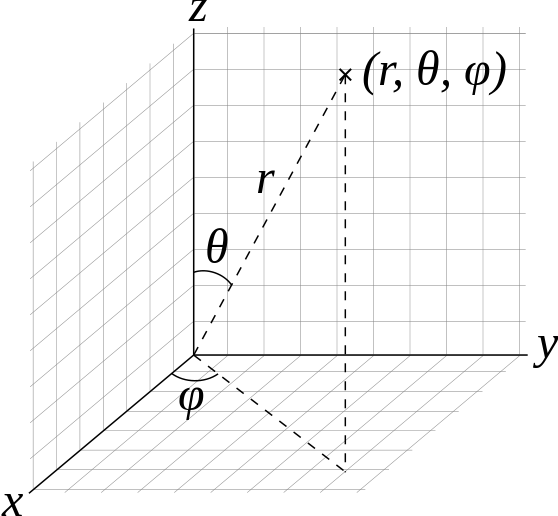
\includegraphics[scale=0.25]{images/sphereCoords}\\
	\tiny{Source: Public Domain, CC0}
	\caption{3D spherical coordinate system}
	\label{fig}
\end{figure}

Uniformly placing points at a fixed radial distance and constant intervals within constrained angles give a collection of points that represent hair roots of the scalp. Increasing the number of hair roots allows sampling of higher fidelity. However, this also demands greater computational resources.

\begin{figure}[!h]
	\centering
	\caption{Sphere meshes visualise root positions. The angle ranges specify coverage area of the scalp, while the interval of placements determines resolution. Fitting a sphere to the reference head mesh approximates the radial distance and origin.}
	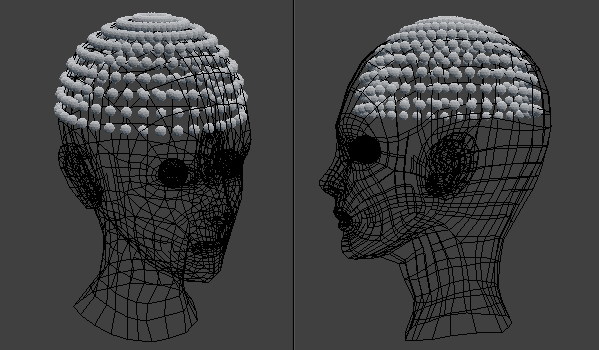
\includegraphics[scale=0.5]{images/spherePoints}\\
	\label{fig}
\end{figure}

A total of 342 splines in our generative model is used to describe hair structure. We construct each spline from 10 points in a 3D space. The resulting feature vector is 10260 dimensions long.

\section{Approximating Generative Parameters from Input Data}
\subsection{Parsing OBJ File}
Approximation begins by parsing the geometric data of OBJ files into a graph data structure of nodes and edges. The axis of exported OBJ files is different from the axis of Blender, to align the coordinate system, swap the Y and Z axis, then negate the Y axis.

\begin{algorithm}[!h]
	\caption{Parsing OBJ format}
	\textbf{Input}: file name\;
	\textbf{Output}: vertex dictionary of 3D points, mesh graph\;
	\For{line \textbf{in} file}{
		\If{line starts with "v "}{
			parse vertex data\;
			add new vertex to vertex dictionary
			add new vertex to graph
		} \ElseIf{line starts with "f "}{
			parse face data\;
			extract edges from new face\;
			add edges to graph\;
		}
	}
	\Return vertex dictionary, graph
\end{algorithm}

\subsection{Spline Estimation}
\subsubsection{Edge Loop Extraction}
The versatile structure of polygon meshes allows it to be an expressive format, however, this flexibility can cause ambiguity when analysing geometric structure. We assume that the mesh only contains sub-meshes of hair segments that have grid-like topology. Our assumption allows us to extract edge loops that describe the structure of hair segments.

In the technical documentation of Blender, it describes an algorithm for edge loop selection. \cite{blenderedgeloop}:
\begin{enumerate}
\item Given a starting edge, only continue searching adjacent edges if the candidates connect to exactly three other neighbours, as any other value would indicate either the border of a mesh or encountering a pole vertex.
\item Completing a cyclic edge loop ends the selection process.
\item Adjacent edges that share a face with the current one are discarded from consideration.
\end{enumerate}
We devise an edge loop extraction algorithm that achieves the properties specified, illustrated in figure \ref{edgeLoopFig}.

\begin{figure}[!h]
	\centering
	\caption{Our edge loop extraction algorithm begins by selecting an edge within the mesh graph. The two vertices of the edge are \textbf{end vertices}. We then proceed to \textit{grow} the edge loop selection. Take the set of \textbf{first degree neighbours} of the \textit{end vertices}, these nodes are the \textit{candidates} for the edge loop. We remove edges that are part of the current edge loop from this set of first degree neighbours. We add the first degree neighbours to a set of face vertices for following iterations. Take the neighbours of the first degree neighbours as a set of \textbf{second degree neighbours}, removing its originating end vertex. A candidate node is only accepted to the edge loop if its set neighbours do not intersect with the set of face vertices. Accepted vertices are appended to the list of end vertices, this process is repeated until there are no end vertices left to grow the selection.}
	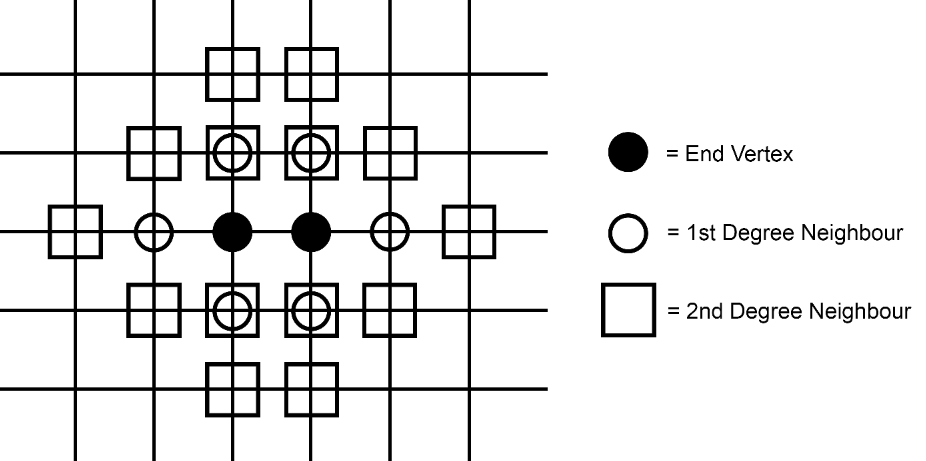
\includegraphics[scale=0.35]{images/edgeLoopDiagram}\\
	
	\label{edgeLoopFig}
\end{figure}

\subsubsection{Border Edge Loops}
Hair structure estimation begins by splitting the mesh into sub-meshes, determined by graph connectivity. For each segment mesh, we are interested in the edge loops that represent hair strands from the scalp roots. To find these edge loops, we must locate the border edge loops of the mesh and choose one to be the root edge loop.

\begin{algorithm}[!h]
	\caption{Extracting border edge loops}
	\While{number of corner vertices greater than 0}{
		pick a corner vertex\;
		\For{vertex in neighbours of selected corner}{
			\If{vertex in set of border or corner vertices}{
				extract edge loops\;
				add edge loops to border edge loops collection\;
				remove vertices of extracted loops from border vertices\;
			}
		}
		\For {vertex in corner vertices}{
			\If{all adjacent border edges of corner vertex have been removed}{
				remove corner vertex\;
			}
		}
	}
	\Return border edge loops
\end{algorithm}

Corner vertices are nodes that have exactly two edges, while border vertices have three edges. Border edge loops are determined by selecting an edge of a corner vertex and growing the edge loop. Any edge of a corner vertex will connect to a border vertex. The selection is specified to stop upon encountering another corner vertex, resulting in an edge loop of a border. We discard the vertices of the extracted border edge loop. Remove any corner vertices that no longer have any neighbours left in the set of border vertices. Repeat until there are no corner nodes left, thus successfully extracting the boundary of the mesh as a collection edge loops.

\begin{figure}[!h]
	\centering
	\caption{Observe that the corner vertices have two edges, and the border edges have three. Determining the root edge loop is done by choosing the border edge loop that is closest to the scalp surface.}
	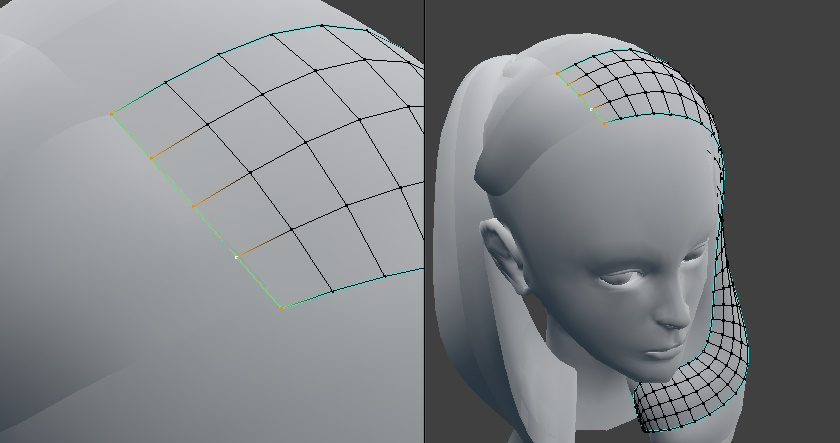
\includegraphics[scale=0.5]{images/rootLoop}\\
\end{figure}

\subsubsection{Root Edge Loop}
The \textit{root edge loop} is the border edge loop that is closest to the surface of the scalp. It serves as a reference for where the hair strands begin. We determine the root loop by finding the average distance of each vertex in a border loop. Heuristically, the root border has minimal distance when aligned across the scalp.

There is a significant flaw in this approach as it will not correctly predict roots of hair segments that are represented by multiple meshes. A solution to this would be to accept hair that has clear roots first then iteratively join \textit{floating segments} to the end of the closest corresponding \textit{rooted segment} until there are no more, or the system is unable to connect any segments further.	

\begin{algorithm}[!h]
	\caption{Determining root border edge loop}
\end{algorithm}

\subsubsection{Pivotal Strand Splines}
With the root loop, we can extract a collection of edge loops that represents the \textit{pivotal} (descriptive) hair strands of the segment cluster. Given the neighbours of root vertices, removing the neighbours that are also root vertices leave edges that represent key strands. When there is one edge, we take the edge loop as a pivotal strand representation. The edge loop will extend until it encounters a pole or ends on the boundary. It is useful to know where the strand starts (from the root), and where it ends. We extract a path from the edge loop graph by continually appending adjacent nodes, starting from the root node. The result forms a spline of connected lines.

\begin{algorithm}[!h]
	\caption{Extracting spline edge loops}
\end{algorithm}

\begin{algorithm}[!h]
	\caption{Reconstructing spline path}
\end{algorithm}

\subsubsection{Spline Repair Operation}
A repair operator processes the strand splines to improve the approximation. First, the starting point of floating splines is attached to the nearest end of a rooted spline if there is one within a specified vicinity. We discard the remaining floating splines that are not attached. Secondly, removing splines that are insignificantly short in length allows for more descriptive splines to be sampled.

\subsubsection{Parametrising a Strand Spline}
The procedure thus far returns a set of strand splines that have varying number of nodes. We produce a constant dimension through sampling to acquire a spline that is applicable for use as parameters of our generative model.

First establish intervals of the distance covered between the points of the original spline. Now suppose we want to evenly sample the spline with $n$ points, we can compute the distance where the $i_{th}$ sample point should travel along the spline as
$$distance=\frac{i \cdot s_l}{n},$$
where $s_l$ is the spline length.

We determine the indices $[j, j+1]$ where the sample distance lies on the spline by comparing the sample distance to the distance of the interval list. The position, $\bm{P}$, of the sample point is
$$\bm{P} = \bm{S} + r\bm{D},$$
where $\bm{S}$ denotes the starting position that is the $j_{th}$ point of the original spline, plus the unit vector direction to the next $j+1_{th}$ point, multiplied by scalar $r$, the remaining distance to cover from the $j_{th}$ interval.

A potential improvement for parametrising the strand splines is to concentrating more sampling points at curves rather than evenly spaced. Using less parameters mitigates problems introduced by the curse of dimensionality.

\subsection{Structure Estimation}
\subsubsection{Selection Operator}
Each root is associated to a spline by a selection operator. Attributes that make a spline more desirable to a particular root are attributes such as proximity or uniqueness compared to previously selected splines. The motivation is to use a set amount of roots to represent the hair structure without losing too much information.
\begin{itemize}
	\item Closest strand to root
	\item Average of area
	\item "Unique" factor
\end{itemize}

\section{Learning a Manifold with Bayesian GP-LVM}

\subsection{Handling Uncertainty}
Add offset so top of head is "mean", so uncertain hair moves towards the top (avoids hair moving inside head or other unlikely areas)

\subsection{GP-LVM and Bayesian GP-LVM}

\subsection{Kernel: ARD, Variance, and Lengthscale}
\subsubsection{RBF}
Smooth
\subsubsection{Exponential}
Moving latent variables make little change when uncertain

\subsubsection{Linear}
Bad, moving in 1 dimensions only changes the hairstyle one way

\section{Generation of Output}
GPy native matplotlib conflicts with Blender as TKInter is disabled.
Plot image of latent space to be imported into image editor of Blender.
Pickle model to be imported by Blender's python.
Select latent variables from manifold (Blender event API)
Read model and predict output by selected latent variables
Generate guide splines following format of latent model and generative model
Extrude by spline object
Rotate by head surface normals
Convert to Poly

\section{Data Acquisition}
Split tests to 0-9 output in folder with user identifier and test value

\section{Challenges}
Discuss problems resolved here

\section{Project Management}
\subsection{Source Control}
Git is used for source control of the project implementation. The branching feature is useful for separating development of features. Maintaining multiple versions of the code base prevented issues caused by the interaction of incomplete features. The merging and rebasing tools helped conflict resolution. Descriptive atomic commits keep a log of progress and supports roll-back to older versions when necessary. A private repository backup was set up on a hosting service provider to prevent data loss and enable development on multiple machines with ease.

\subsection{Issue Tracking}
Trello

\subsection{Time-line}
Calender.
Internal Deadlines.

\begin{table}[!h]
	\centering
	\begin{tabular}{|cc|c|}
		\hline
		foo      & bar      & baz      \\
		\hline
		$0     $ & $0     $ & $0     $ \\
		\hline
	\end{tabular}
	\caption{This is an example table.}
	\label{tab}
\end{table}

% -----------------------------------------------------------------------------

\chapter{Critical Evaluation}
\label{chap:evaluation}

\section{Functional Testing}
functional  testing, including analysis and explanation of failure cases.

bald spots, inside head, intersection 
causes and solutions

3 pages


\section{Behavioural Testing}
behavioural testing, often including analysis of any results that draw some form of conclusion wrt. the aims and objectives

questionnaire analysis

3 pages

\section{Statistical Analysis}
null hypothesis, type 1-2 err, t-tests, empirical methods (see gmail), etc

1 pages

\section{Evaluation}
evaluation of options and decisions within the project, and/or a comparison with alternatives.
5 page

\subsection{Training and Model}
Assumes training data is correct. Triangles are a problem.
Approximating loses a lot of data, data that is manually converted provides more information, giving better output visually.

Works better when styles are similar, otherwise strands interpolate in between to be incorrect such as inside head.

\subsection{Choice of Learning Model}
Linear, decision trees, neural nets, GPLVM
Supervised, unsupervised, genetic

\subsection{Comparing with Other methods}
AutoHair, Exemplar, etc

\subsection{Extending to other models}
Simulating foliage, grass.
Can easy do surface
Combine models
Deep GPs
2 pages

\subsubsection{Addressing Non-Intuitive Use}
Plot small image of output in corresponding area of latent variable model to illustrate the certain areas (training data) so users can explore around it for variation.

\subsubsection{Observations}
What I can do:
transferring to fixed objects like a face: mouth, eye, etc that is more "predictable".

\section{Applications}
MMOs, games, etc.
3D latent space with VR.
2 page

% -----------------------------------------------------------------------------

\chapter{Conclusion}
\label{chap:conclusion}

\section{Summary}
(Re)summarise the main contributions and achievements, in essence
summing up the content. 2 pages

\section{Project Status}
Clearly state the current project status (e.g., ``X is working, Y 
is not'') and evaluate what has been achieved with respect to the 
initial aims and objectives (e.g., ``I completed aim X outlined 
previously, the evidence for this is within Chapter Y'').  There 
is no problem including aims which were not completed, but it is 
important to evaluate and/or justify why this is the case. 2 pages

\section{Future Work}
Outline any open problems or future plans.  Rather than treat this
only as an exercise in what you {\em could} have done given more 
time, try to focus on any unexplored options or interesting outcomes
(e.g., ``my experiment for X gave counter-intuitive results, this 
could be because Y and would form an interesting area for further 
study'' or ``users found feature Z of my software difficult to use,
which is obvious in hindsight but not during at design stage; to 
resolve this, I could clearly apply the technique of Smith [7]''). 1 page



% =============================================================================

% Finally, after the main matter, the back matter is specified.  This is
% typically populated with just the bibliography.  LaTeX deals with these
% in one of two ways, namely
%
% - inline, which roughly means the author specifies entries using the 
%   \bibitem macro and typesets them manually, or
% - using BiBTeX, which means entries are contained in a separate file
%   (which is essentially a databased) then inported; this is the 
%   approach used below, with the databased being dissertation.bib.
%
% Either way, the each entry has a key (or identifier) which can be used
% in the main matter to cite it, e.g., \cite{X}, \cite[Chapter 2}{Y}.

\backmatter

\bibliography{dissertation}

% -----------------------------------------------------------------------------

% The dissertation concludes with a set of (optional) appendicies; these are 
% the same as chapters in a sense, but once signaled as being appendicies via
% the associated macro, LaTeX manages them appropriatly.

\appendix

\chapter{An Example Appendix}
\label{appx:example}

Content which is not central to, but may enhance the dissertation can be 
included in one or more appendices; examples include, but are not limited
to

\begin{itemize}
	\item lengthy mathematical proofs, numerical or graphical results which 
	are summarised in the main body,
	\item sample or example calculations, 
	and
	\item results of user studies or questionnaires.
\end{itemize}

\noindent
Note that in line with most research conferences, the marking panel is not
obliged to read such appendices.

% =============================================================================

\end{document}
